\documentclass[preprint]{sigplanconf}
%\documentclass{sig-alternate}
\usepackage{epsfig, times, graphicx, amssymb, amsmath, amsfonts}

\newcommand{\mt}[1]{\mbox{\it #1}}

\begin{document}

\conferenceinfo{LCTES'05,} {June 15--17, 2005, Chicago, Illinois, USA.}
\CopyrightYear{2005}
\copyrightdata{1-59593-018-3/05/0006} 

\title{Cache Aware Optimization of Stream Programs}
\authorinfo{Janis Sermulins \and William Thies \and Rodric Rabbah \and Saman Amarasinghe}
	     {Computer Science and Artificial Intelligence Laboratory, Massachusetts Institute of Technology}
	     {\{janiss, thies, rabbah, saman\}@csail.mit.edu}

\maketitle

\begin{abstract}
As DSP programming is becoming more complex, there is an increasing
need for high-level abstractions that can be efficiently compiled.
Toward this end, we present a set of aggressive optimizations that
target linear sections of a stream program.  Our input language is
StreamIt, which represents programs as a hierarchical graph of
autonomous filters.  A filter is linear if each of its outputs can be
represented as an affine combination of its inputs.  Linear filters
are common in DSP applications; examples include FIR filters,
expanders, compressors, FFTs and DCTs.

We present a linear extraction analysis that automatically detects
linear filters based on the C-like code in their {\tt work} function.
Once linear filters are identified, we show how neighboring nodes can
be collapsed into a single linear representation, thereby eliminating
many redundant computations.  Also, we describe a method for
automatically translating linear nodes into the frequency domain,
thereby yielding algorithmic savings for convolutional filters.

We have completed a fully-automatic implementation of the above
techniques as part of the StreamIt compiler, and we demonstrate
performance improvements that average 400\% over our benchmark
applications.




\end{abstract}

\category{D.3.4}{Programming Languages}{Processors}[Optimization; code generation; compilers]
\category{D.3.2}{Programming Languages}{Language Classifications}[Concurrent, distributed, and parallel languages; Data-flow languages]
%\category{D.2.2}{Software Engineering}{Software Architectures, Design Tools and Techniques}

\terms 
Languages, Design, Performance

\keywords
Stream Programing, StreamIt, Synchronous Dataflow, Cache, Cache
Optimizations, Fusion, Embedded

%\section{Introduction}

Applications that are structured around some notion of a ``stream''
are becoming increasingly important and widespread.  There is evidence
that streaming media applications are already consuming most of the
cycles on consumer machines \cite{Rix98}, and their use is continuing
to grow.  In the embedded domain, applications for hand-held
computers, cell phones, and DSP's are centered around a stream of
voice or video data.  The stream abstraction is also fundamental to
high-performance applications such as intelligent software routers,
cell phone base stations, and HDTV editing consoles.

Despite the prevalence of these applications, there is surprisingly
little language and compiler support for practical, large-scale stream
programming.  Of course, the notion of a stream as a programming
abstraction has been around for decades \cite{SICP}, and a number of
special-purpose stream languages have been designed (see
\cite{survey97} for a review).  Many of these languages and
representations are elegant and theoretically sound, but they often
lack features and are too inflexible to support straightforward
development of modern stream applications, or their implementations
are too inefficient to use in practice.  Consequently, most
programmers turn to general-purpose languages such as C or C++ to
implement stream programs.

There are two reasons that general-purpose languages are inadequate for
stream programming.  Firstly, they are a mismatch for the application
domain.  That is, they do not provide a natural or intuitive
representation of streams, thereby having a negative effect on
readability, robustness, and programmer productivity.  Moreover, because
the widespread parallelism and regular communication patterns of data
streams are left implicit in general-purpose languages, compilers are
not stream-conscious and do not perform stream-specific optimizations.
As a result, performance-critical loops are often hand-coded in a
low-level assembly language and must be re-implemented for each target
architecture.  This practice is labor-intensive, error-prone, and very
costly.

Secondly, general-purpose languages are a mismatch for the emerging
class of grid-based architectures \cite{smartmemories,rawshort,trips} that
are especially well-suited for stream processing.  Perhaps the primary
appeal of C is that it provides a ``common machine language'' for
von-Neumann architectures.  That is, it abstracts away the
idiosyncratic differences between machines, but encapsulates their
common properties: a single program counter, arithmetic operations,
and a monolithic memory.  However, for grid-based architectures, the
von-Neumann model no longer holds, as there are multiple instruction
streams and distributed memory banks.  Thus, C no longer serves as a
common machine language--in fact, it provides the wrong abstraction
for the underlying hardware, and architecture-specific directives are
often needed to obtain reasonable performance.  Again, this greatly
complicates the job of the programmer and hampers portability.

StreamIt is a language and compiler specifically designed for modern
stream programming.  The StreamIt language has two goals: first, to
provide high-level stream abstractions that improve programmer
productivity and program robustness within the streaming domain, and
second, to serve as a common machine language for grid-based
processors.  At the same time, the StreamIt compiler aims to perform
stream-specific optimizations to achieve the performance of an expert
programmer.

This paper motivates, describes, and justifies the high-level language
features of StreamIt, version 1.0.  The major limitation of StreamIt
1.0 is that all flow rates in the streams must be static; applications
such as compression that have dynamically varying flow rates will be
the subject of future work.  A large set of applications can be
implemented with static rates, and while dynamic rates will require a
different runtime model, it will still be essential to fully analyse
and optimize static sub-sections in order to obtain high performance.

The paper is organized as follows. In Section {\ref{sec:domain}}, we
characterize the domain of streaming programs that motivates the
design of StreamIt, and in Section~\ref{sec:overview} we describe the
language features in detail.  We present an in-depth example of a
software radio in Section~\ref{sec:example}, preliminary results in
Section~\ref{sec:results}, related work in Section~\ref{sec:related},
and conclusions in Section~\ref{sec:conc}.


\section{Introduction}

Efficiency and high performance are of central importance within the
embedded domain.  As processor speeds continue to increase, the memory
bottleneck remains a primary impediment to attaining performance.
Current practices for hiding memory latency are invariably expensive
and complex.  For example, superscalar processors resort to
out-of-order execution to hide the latency of cache misses.  However,
this results in large power expenditures (unfit for embedded systems)
and also increases the cost of the system.  Compilers have also
attempted aggressive optimizations for the memory hierarchy, but this
has proven to be impossibly complex due to the obscured parallelism
and communication patterns in traditional languages such as C.

For performance-critical programs, the complexity inevitably
propagates all the way to the application developer.  Programs are
written to explicitly manage parallelism and to reorder the
computation so that the instruction and data working sets fit within
the cache.  For example, the inputs and outputs of a procedure might
be arrays that are specifically designed to fit within the data cache
on a given architecture; loop bodies are written at a level of
granularity that matches the instruction cache.  While manual tuning
can be effective, the end solutions are not portable.  They are also
exceedingly difficult to understand, modify, and debug.

The recent emergence of streaming applications represents an
opportunity to mitigate these problems using simple transformations in
the compiler.  Streaming codes encompass a broad spectrum of
applications, including embedded communications processing, multimedia
encoding and playback, compression, and encryption.  They also range
to server applications, such as HDTV editing and hyper-spectral
imaging.  Stream programs are rich with parallelism and regular
communication patterns that can be exploited by the compiler to
automatically tune memory performance.  It is natural to express a
stream program as a high-level graph of independent components, or
{\it actors}.  Actor communicate using explicit FIFO channels and can
execute whenever a sufficient number of items are available on their
input channels.  In a stream graph, actors can be freely combined and
reordered to improve caching behavior so long as there are sufficient
inputs to complete each execution.  These transformations serve to
automate tedious approaches that must be performed manually using
today's languages; they are too complex to perform automatically in
hardware or in the most aggressive of C compilers.

%By calculating the input and
%output rates of each actor, the compiler can determine how long to
%execute each one so as to assure that the outputs fit within the data
%cache.  In addition, by running an actor multiple times in succession,
%instruction locality is enhanced.  

This paper presents three simple cache aware optimizations for stream
programs: {\it (i)} execution scaling, {\it (ii)} cache aware fusion,
and {\it (iii)} scalar replacement.  These optimizations represent a
{\it unified approach} that simultaneously considers the instruction
and data working sets.  We also develop a simple quantitative model of
caching behavior for streaming workloads, providing a foundation to
reason about the transformations.  Our work is done in the context of
the Synchronous Dataflow~\cite{LM87-i} model of computation, in which
each actor in the stream graph has a known input and output rate.  This
is a popular model for a broad range of signal processing and embedded
applications.

Execution scaling is a transformation that improves instruction
locality by executing each actor in the stream graph multiple times
before moving on to the next actor.  As a given actor usually fits
within the cache, the repeated execution serves to amortize the cost
of loading the actor from off-chip memory.  However, as our cache
model will show, actors should not be scaled excessively, as their
outputs will eventually overflow the data cache.  We present a simple
and effective algorithm for calculating a scaling factor that respects
both instruction and data constraints.

Prior to execution scaling, pairs of actors that both fit in the
instruction cache are optimized using cache aware fusion.  Fusion
combines several actors into one, thereby eliminating function calls
and allowing the compiler to optimize across actor boundaries.
However, as fusion combines actors into a single function, it has the
potential to exceed the instruction cache.  Our cache aware fusion
algorithm only fuses actors as long as they do not jeopardize
instruction locality.

As actors are fused together, new buffer management strategies become
possible.  The most aggressive of these, termed scalar replacement,
serves to replace an array with a series of local scalar variables.
Unlike array references, scalar variables can be register allocated,
leading to large performance gains.  We also develop a new buffer
management strategy (called ``copy-shift'') that extends scalar
replacement to sliding-window computations, a domain where complex
indexing expressions typically hinder compiler analysis.

Our cache aware optimizations are implemented as part of StreamIt, a
language and compiler infrastructure for stream
programming~\cite{streamitcc}.  We evaluate the optimizations on three
architectures.  The StrongARM 1110 represents our primary target; it
is an embedded processor without a secondary cache.  Our other targets
are the Pentium~3 (a superscalar) and the Itanium~2 (a VLIW
processor).  We find that execution scaling, cache aware fusion, and
scalar replacement each offer significant performance gains, and the
most consistent speedups result when all are applied together.
Compared to unoptimized StreamIt code, our cache optimizations yield a
249\% speedup on the StrongARM, a 154\% speedup on the Pentium~3, and
a 152\% speedup on Itanium~2.  These numbers represent averages over
our streaming benchmark suite.

This paper is organized as follows.  Section~2 gives background
information on the StreamIt language.  Section~3 lays the foundation
for our approach by developing a quantitative model of caching
behavior for any sequence of actor executions.  Section~4 describes
execution scaling and cache-aware scheduling.  Section~5 evaluates
buffer management strategies within fused actors, including scalar
replacement.  Section~6 contains our experimental evaluation of these
techniques in the StreamIt compiler.  Finally, Section~7 describes
related work and Section~8 concludes.

%% In summary, this paper presents a unified optimization strategy for
%% improving instruction and data locality.  Its contributions are:
%% \begin{itemize}
%% \item A cache model for stream computing that provides a quantitative
%% estimate of the caching performance for any sequence of actor
%% executions (Section 3).
%% \item A cache aware scheduling heuristic that judiciously scales the
%% execution frequency of actors to improve instruction and data locality,
%% while not overflowing the data cache (Section 4).
%% \item A cache aware partitioning policy that judiciously fuses
%% adjacent actors into a single component, enabling local optimizations,
%% while not overflowing the instruction cache (Section 4).
%% \item An optimized buffer management policy, termed ``copy-shift with
%% execution scaling'', which out-performs a traditional rotating buffers
%% in a micro-benchmark analysis (Section 5).
%% \item An evaluation of these techniques using the
%% StreamIt compiler and a streaming benchmark suite of eleven programs.
%% Compared to unoptimized StreamIt, the cache optimizations deliver an
%% average speedup of 249\% on a StrongARM, 154\% on a Pentium~3 and
%% 152\% on an Itanium~2 (Section 6).
%% \end{itemize}

%% In traditional C programs, the compiler is very good at generating
%% code within a function to keep resources busy when there is available
%% ILP.  However, with current language abstractions, it is extremely
%% difficult for the compiler to do large-scale reordering of different
%% parts of the program to match a given data cache.  This is because a)
%% the coarse-grained data dependences are not exposed, limiting
%% reordering opportunities, b) data access patterns are obscured, making
%% it hard to predict what should be cached, and c) the communication
%% pattern and bandwidth between components is obscured, often through
%% shared memory.
%%
%% As a result, programmers have turned to manually optimizing a
%% streaming runtime system to fit a given cache hierarchy.  Procedures
%% are written in terms of a given block size that leads to good data
%% caching behavior.  This block size is propagated throughout the
%% program and becomes inseparable with the underlying algorithm.  When
%% the architecture changes, the code must be re-engineered to suite the
%% new caching system.  It also becomes very complex from the
%% programmer's standpoint, as the high-level algorithm is lost in the
%% details.
%%
%% The recent emergence of streaming applications (examples) represents a
%% new opportunity for the compiler to achieve good use of the cache
%% hierarchy using simple high-level transformations.  A stream program
%% is often represented as a graph of independent actors, where all
%% communication between actors occurs over explicit FIFO queues.  Actor
%% executions can be reordered so long as they respect the data
%% dependences over the communication channels.  By calculating the input
%% and output rates of each actor, the compiler can determine how long to
%% execute each one so as to assure that the working set remains in the
%% cache.  In addition, by running each actor for as long as possible at
%% a given time, instruction locality is enhanced.  These transformations
%% serve to automate tedious approaches that have must be performed
%% manually using today's languages and compilers.

\section{StreamIt}
\label{sec:streamit}

StreamIt  is   an  architecture independent language that is
designed for  stream programming. In StreamIt, programs are
represented as graphs where  nodes represent  computation and edges
represent FIFO-ordered communication of data over tapes.

\paragraph*{Hierarchical Streams}
In  StreamIt, the  basic programmable  unit (i.e., an actor) is a {\it
filter}.   Each filter contains  a work  function that executes
atomically,  popping (i.e., reading)  a fixed number  of items  from
the  filter's input  tape and pushing (i.e., writing) a fixed number
of items to the filter's output tape.  A filter  may also {\tt peek} at
a given index  on its input tape without  consuming  the  item;  this
makes  it  simple  to  represent computation over a
sliding window.   The {\tt push}, {\tt pop}, and {\tt peek} rates are
declared as part  of  the work  function,  thereby enabling  the
compiler    to construct a static schedule of filter executions. The
following is an example implementation of a Finite Impulse
Response (FIR)  filter: 

\begin{scriptsize}
% {\small
\begin{verbatim}
float->float filter FIR (int N, float[] weights) 
{
  work push 1 pop 1 peek N {
    float sum = 0;
    for (int i = 0; i < N; i++) {
      sum += peek(i) * weights[i];
    }
    pop();
    push(sum);
  }
}
\end{verbatim}
% }
\end{scriptsize}

The work function is invoked (fired) whenever there is sufficient data
on the input tape. For the FIR example above, the filter requires at least
\texttt{N} elements before it can execute. The value of \texttt{N} is
known at compile time when the filter is composed to form a stream
graph. A filter is akin to a class in object oriented programming
with the work function serving as the main method. The parameters
to a filter (e.g., \texttt{N} and \texttt{weights}) are equivalent to
parameters passed to a class constructor. 

\begin{figure}[t]
\begin{center}
%\vspace{-24pt}
% \framebox{
 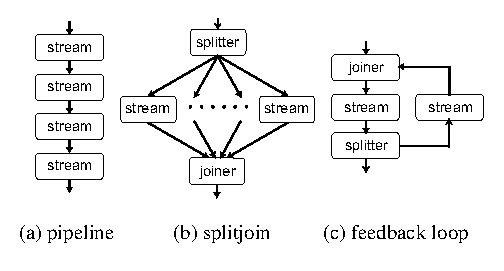
\includegraphics[scale=1, angle=0]{./constructs-eg.eps}
%}
% \vspace{-6pt}
% \nocaptionrule
 \caption{Hierarchical streams in StreamIt.}
 \label{fig:containers}
\end{center}
\end{figure}

\begin{figure}[t]
\begin{center}
\vspace{-12pt}
% \framebox{
 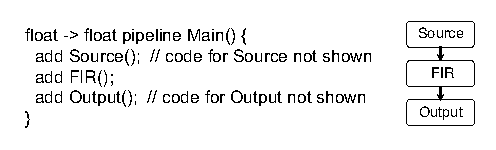
\includegraphics[scale=1, angle=0]{./pipeline-eg.eps}
%}
% \vspace{-6pt}
% \nocaptionrule
 \caption{Example pipeline with FIR filter.}
 \label{fig:pipeline}
%\vspace{-18pt}
\end{center}
\end{figure}

In StreamIt, the
application developer focuses on the hierarchical assembly of the
stream graph and its communication topology, rather than on the 
explicit management of the data buffers between filters.
StreamIt provides three hierarchical structures for composing filters
into larger stream graphs (see Figure~\ref{fig:containers}). The 
{\it pipeline} construct composes streams in sequence, with the output
of one connected to the input of the next.   An example of a pipeline
appears in Figure~\ref{fig:pipeline}.

The {\it splitjoin} construct distributes data to a set of parallel
streams, which are then joined together in a round robin fashion.  In
a splitjoin, the {\it splitter} performs the data scattering, and the
{\it joiner} performs the gathering. A splitter is a specialized
filter with a single input and  multiple output channels. On 
every execution step, it can distribute its output to any one of
its children in either a {\it duplicate} or a {\it roundrobin}
manner. For the former, incoming data are replicated to every
sibling connected to the splitter. For the latter, data are scattered
in a round robin manner, with each item sent to exactly one child
stream, in order.  The splitter type and the weights for distributing data to
child streams are declared as part of the syntax (e.g., \texttt{split
duplicate} or \texttt{split roundrobin($w_1,\ldots,w_n$)}). The
splitter counterpart is the joiner. It is a specialized filter with  
multiple input channels but only one output channel. The joiner
gathers data from its predecessors in a round robin manner (declared
as part of the syntax) to produce a single output stream.

StreamIt also provides a {\it feedback loop} construct for introducing
cycles in the graph.

%\section{Execution Model}
%\label{sec:execmodel}

%% A StreamIt program is represented by a hierarchical graph,
%% where the leaf nodes are filters, splitters, and joiners, and
%% the composite nodes are pipelines, splitjoins, and
%% feedback-loops. Edges in the graph represent data channels, which 
%% operate as FIFO queues.
\paragraph*{Execution Model}
As noted earlier, an actor (i.e., a filter, splitter, or joiner)
executes whenever there are enough data items on its input 
tape. In StreamIt, actors have  two epochs
of execution: one for initialization, and one for the {\it steady
state}. The initialization primes the input tapes to allow filters with
peeking to execute the very first instance of their work functions.
%%initialization in this setting is similar to the prologue stage in
%%software pipelining. 
A steady state is an execution that does not change the
buffering in the channels: the number of items on each channel
after the execution is the same as it was before the execution. 
Every valid stream graph has a steady state~\cite{LM87-i}, and within
a steady state, there are often many possibilities for interleaving
actor executions. 
%% The steady state schedule has the property that
%% the amount of data buffered between any two actors does not change
%% before and after the actor executions.
\begin{figure}[t]
\begin{center}
%%\vspace{-24pt}
%\vspace{24pt}
 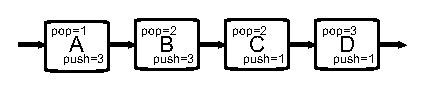
\includegraphics[scale=1, angle=0]{./pipe-with-rates.eps}
%\vspace{-6pt}
% \nocaptionrule
 \caption{Example pipeline.}
 \label{fig:pipe-with-rates}
\end{center}
%\vspace{-12pt}
\end{figure}
An example of a steady state for the pipeline in
Figure~\ref{fig:pipe-with-rates} requires filter \texttt{A} to fire
4 times, \texttt{B} 6 times, \texttt{C} 9 times, and
\texttt{D} 3 times. 
% Because in StreamIt the filters are
% independent (i.e., they do not share state), they can execute
% concurently. In a uniprocessor setting (which is what we use for our
% evaluation), we can only run one filter at time. Therefore, 
% The data generated by one actor are buffered (cached) until they are
% consumed.

\paragraph*{Compilation Process}
The StreamIt compiler derives the initialization and steady state
schedules~\cite{karczma-lctes03} and outputs a C program that includes
the initialization and work functions, as well as a driver to execute
each of the two schedules. Our compilation process allows the StreamIt
compiler to focus on high level optimizations, and relies on existing
compilers to perform machine-specific optimizations such as register
allocation, instruction scheduling, and 
code generation---this two step approach affords us a
great deal of portability (e.g., code generated from the StreamIt
compiler is compiled and run on three different machines as reported
in Section~\ref{sec:evaluation}).

%% For example, referring to
%% Figure~\ref{fig:pipe-with-rates}, the compiler generates the following
%% sample code for running the steady state schedule:
%% %\begin{scriptsize}
%% \begin{verbatim}
%% run_steady_state() {
%%   for (i = 0; i < 4; i++) A_work();
%%   for (i = 0; i < 6; i++) B_work();
%%   for (i = 0; i < 9; i++) C_work();
%%   for (i = 0; i < 3; i++) D_work();
%% }
%% \end{verbatim}
%% %\end{scriptsize}
%% To execute the program, the steady state is wrapped with
%% another loop that invokes the steady state a designated number of
%% times. Preceding the state steady, a similar initialization schedule
%% is run to prime the data buffers.
%, and following the steady state, an
%epilogue is run to drain the buffers as necessary.

%% \begin{figure}[t]
%% \begin{center}
%% \vspace{-12pt}
%%  \psfig{figure=ssi.eps,width=3in}
%%  \vspace{-6pt}
%%  \caption{Instruction size (in bytes along the y-axis) per filter
%%  (x-axis) occurring in a steady state execution of FFT.}
%%  \label{fig:ssi-single}
%% \vspace{-18pt}
%% \end{center}
%% \end{figure}

\section{Cache Model for Streaming}
\label{sec:cache-model}

In this section we describe a simple and intuitive cache model to
estimate the instruction and data cache behavior given an execution
ordering of the filters in the stream graph.

The model is based on the notion of a filter reuse distance which is 
based on LRU stack distance~\cite{mattson70}. We develop the model
first for the instruction cache, and then subsequently generalize it to
account for the data cache.

\subsection{Instruction Cache}

A {\it filter execution trace} is a sequence of 
filter work functions executions: $T = f_0 f_1 ... f_n$; $f_i$ represents the
execution of filter $f$ at logical time $i$.
The filter {\it instruction reuse distance} ($IRD$) is defined as the
number of unique instructions that are referenced between two
instances of the same work function. Formally, we define $phase(f_i)$
as the sequence $f_i ... f_l$ ($i < l$) of work functions occurring in
$T$ such that $f_i = f_l$ and no where else (i.e., $f_i \neq f_k$
$\forall{k}~~s.t.~~i < k < l$). The $IRD(f_i) = \sum I(f_j)$ over all
distinct filters occurring in $phase(f_i)$, and $I(f)$ equals the code
size of a filter $f$. Based on this reuse metric, we define an
instruction-cache-miss step function $ICM(f_i)$ such that:
\begin{equation}
\label{eq:icm}
  ICM(f_i) =
    \begin{cases}
      0& \text{if $IRD(f_i) \leq C_I$; hit/no cache refill},\\
      1& \text{else; a miss/(some) cache refill}.\\
    \end{cases}
\end{equation}
Note that if $f_i$ is the last occurrence of a filter $f$ in the trace,
then $ICM(f_i) = 0$. In Equation~\ref{eq:icm}, $C_I$ represents a
constant proportional to the instruction cache size.

We do not account for the cold start
effects of an execution trace. This does not effect our model, and can
be easily remedied if necessary. To see why this is so, consider the
following two execution traces which represent the executions of work
functions for two filters \texttt{A} and \texttt{B}:
$T_1 = \texttt{A}_1\texttt{A}_2\texttt{B}_3\texttt{B}_4$
and 
$T_2 = \texttt{A}_1\texttt{B}_2\texttt{A}_3\texttt{B}_4$.
In both 
traces, the number of cold starts is the same (i.e., two in all).

What our reuse metric quantifies is the number of misses when a specific work
function is reinvoked. For example, assume that each filter is of the exact
size: $I(\texttt{A}) = I(\texttt{B}) = \lceil{C_I / 2}\rceil + 1$;
that is, the combined instruction workingset of both filters exceeds
the instruction cache, although each filter has a code size that is
smaller than the cache size. Naturally, we expect the trace $T_1$ to
suffer one cold start miss and no other misses for filter \texttt{A}
(and similarly for the other filter). Our model is in accord with
intuition:  $ICM(\texttt{A}_1) = 0$ since
the $IRD(\texttt{A}_1) < C_I$.

In the case of trace $T_2$, we know that since the combined
instruction workingset of the filters exceeds the cache size, when
filter \texttt{B} is invoked following \texttt{A}, it evicts part of
filter \texttt{A}'s instruction workingset. Hence when we transition
back to run filter \texttt{A}, we have to refetch certain
instructions, but in the process, we replace parts of filter
\texttt{B}'s workingset. Hence, we have suffered one cold start miss,
and one capacity miss for filter \texttt{A}, and similarly for
\texttt{B}. Our model is again in accord with intuition: 
$ICM(\texttt{A}_1) = 1$ since
the $IRD(\texttt{A}_1) > C_I$. Note that the
amount of refill is proportional to the number of cache lines that are
replaced when swapping filters, and as such, we may wish to adjust
our cache miss step function. One simple variation is to allow for
some partial replacement without unduly penalizing the overall value
of the metric. Namely, we can allow the constant $C_I$ to be some
fraction greater than the actual cache size. Alternatively, we can use
a more complicated miss function with a more uniform probability
distribution.

Using the metrics above, we can estimate the instruction-cache miss
rate $(IMR)$ as $\sum ICM(f_i)$ over all $f_i$ in the trace, divided
by the size of the trace. Note that different execution orderings for
the same stream graph lead to traces of the same size and hence the
comparisons are fair. The model allows us to rank the quality of an
execution ordering, with scheduling decisions that boost temporal
locality yielding miss rates closer to zero (and schedules that do not
exploit temporal locality yielding traces with miss rates closer to
one).

Our model predicts that scaling is always beneficial from an
instruction-cache point of view. As a reminder, by scaling, we mean
that a filter's work function is run for a greater number of times in
the steady state before transitioning to the next filter in the
graph. Hence for example, a program that would generate a trace $T_2$
might be as follows:
{\small
\begin{verbatim}
run_steady_state() {
  for (i = 0; i < 1; i++) A_work();
  for (i = 0; i < 1; i++) B_work();
}
\end{verbatim}}
but a scaled program that increases temporal locality is as follows:
{\small
\begin{verbatim}
run_steady_state() {
  for (i = 0; i < M * 1; i++) A_work();
  for (i = 0; i < M * 1; i++) B_work();
}
\end{verbatim}}
where \texttt{M} (the multiplicity factor) is an integer greater than
one. From our model, it is easy to see that scaling reduces the number
of misses for a given filter $f$ from $K$ to $\frac{K}{\texttt{M}}- 1$, where $K =
\sum ICM(f)$ for all occurrences of $f$ in  the execution trace.

\subsection{Data Cache}

As noted earlier, we can not arbitrarily scale the execution frequency
of a filter without also considering how scaling might impact
the data buffer sizes between filers. In this regard, a filter's
output buffer size is also constrained by the amount of state that a
filter retains with every execution of its work function.

Clearly if a filter has any static data (e.g., state information or
coefficient arrays), then it is prudent to maximize their temporal
access locality. We can define a data-cache miss rate equation ($DMR$) based on
a derivation similar to that for the instruction-cache miss rate:
replace $C_I$ with $C_D$ in Equation~\ref{eq:icm}, and $I(f_i)$ with
$S(f_i)$ when calculating the {\it data reuse distance} ($DRD$). 
Here, $C_D$ represents a constant proportional to the data cache size,
and $S(f)$ represents the total size of the static data in the
specified filter.

The presence of static data in a filter implies that we have to limit
the scaling of a filter $f$ such that it does not require more than $C_D -
S(f_i)$ bytes of buffer space for reading and writing data; otherwise
the data workingset of the filter will overflow the cache and we lose
produce-consumer locality. The buffer requirements are represented by
$Y(f_i)$, and the data-cache model accounts for the dynamic data
requirements by adjusting the data reuse distance as follows:
$DRD(f_i) = \sum (S(f_i) + Y(f_i))$ over all distinct filters occurring
in $phase(f_i)$.

Intuitively, the dynamic data accounts for the size of the buffer
required for writing new values, as well as the size of the buffer
necessary for reading values. It also adjusts for any
producer-consumer locality since the output buffer of one filter is
also the input buffer of its sibling in the stream graph. What this
measures tells us is that we can scale the execution of a filter as
long as its buffer requirements (for reading and writing) do not
exceed the cache, and furthermore, as long as the input-output rates
between producer consumer pairs are not grossly mismatched. This later
qualification is important and motivates a series of cache
optimizations discussed in the next section. In the case of rate
mismatch, the metric tells us that the effective cache size is
reduced, or in other words, the data that is left over after a
producer-consumer firing must be preserved until a future occurrence of
the same pair of filters. This translates to lower data locality and
degrades cache performance.

Mathematically, the dynamic data measure is defined as:
\begin{eqnarray}
  \nonumber
  Y(f_i) &=&\sum_{f_k} min(W(f_k), U(f_k) \times A(f_k)) + \\
  \nonumber
	   &&\sum_{f_k} min(R(f_k), O(f_k) \times A(f_k)) - \\
  \nonumber
         &&\sum_{f_s} min(R(f_s), O(f_s) \times A(f_s))
\end{eqnarray}
with $W(f)$ equal to the output buffer size reserved for writing data, $R(f)$
equal to the input buffer size reserved for reading data, $U(f)$ equal to the
{\tt push} rate (in bytes) of the filter, $O(f)$ equal to the {\tt pop} rate (in
bytes) of the filter, and $A(f)$ equal to the number of occurrences of
filter $f$ in $phase(f_i)$. Also note that the $Y(f_i)$ is defined
over all distinct occurrences of $f_k$ in the phase, and $f_s$
represents the filter that consumes the data produced by $f_k$ (i.e.,
it is $f_k$'s successor in the stream graph, and $f_k$-$f_s$
constitute a producer-consumer pair; $f_s$ is unique unless $f_k$ is a splitter).

The first term in the equation above quantifies the address space
accessed for writing data. It is  equal to the lesser of the buffer size
reserved for output, and the total number of items produced by
the filter (i.e., the push rate multiplied by the number of times the
work function fired in the phase); this avoids over estimating the
address space when an exceedingly large buffer is reserved but only a
portion of it is used for writing in a phase.

The second term in the equation quantifies the referenced address space 
for reading the input data. This term is also the lesser of two
values: the input buffer size, and the total number of bytes referenced for
reading data.

The third term avoids double counting since the output buffer of one
filter is also the input buffer of its successor in the stream
graph. The term quantifies the amount of data that is consumed by the
producer's successor (which therefore releases a portion of the
address space for use by other filters in the phase).

\subsection{Remarks}

Note  that we can  combine the  instruction and  data cache  miss rate
equations to yield one measure that estimates the temporal locality of
a streaming computation.

Also note that while we use  an execution trace to describe our model,
it  is possible  to  calculate  the instruction  and  data cache  miss
metrics at  compile time.  To do so,  we can leverage  the hierarchical
StreamIt   representation  that  dictates   the  ordering   of  filter
executions.

\section{Cache Optimizations}
\label{sec:cache-opt}

In this section we describe a set of cache-aware transformations that
are geared toward improving the instruction and temporal locality of a
stream graph. We first describe our methodology for scaling actor
firings, and subsequently we describe an optimization that is geared
toward reducing the static and dynamic data requirements of
producer-consumer pairs.

% - multiplicity algorithm
% - forward reference to results

% - partitioning algorithm
% - forward reference to results

\subsection{Multipilicity Scaling}

The goal of this optimization is to increase the execution frequency
of the actors in a steady state schedule, such that the temporal
locality in the memory hiearchy is improved. Our approach is to find a
single multiplicity factor \texttt{M} for scaling all actors, such that
at least 90\% of the actors have a data workingset that fits in the cache.
In other words, using our model, we calculate $M$ such that 
$S(f) + D(f) \leq C_D$ and $DCM(f) = 0$ for 90\% of the actors in the
stream graph.

The algorithm 
computes the largest scaling factor for every actor such that its data
workingset does not exceed the size of the primary data cache
(16~Kb on P3 for example). This yields a set of multiplicities
${\texttt{M}_0, \ldots, \texttt{M}_n}$ for the actors in the stream
graph. For example, the algorithm might calculate
$\texttt{M}_\texttt{A} = 10$,
$\texttt{M}_\texttt{B} = 20$, 
$\texttt{M}_\texttt{C} = 30$, 
$\texttt{M}_\texttt{D} = 40$ for four filters \texttt{A}, \texttt{B},
\texttt{C}, and \texttt{D} in a stream graph.
The algorithm then examines the
distribution and selects the $\texttt{M}_i$
for which 90\% of the actors satisfy our data workingset criterion.
In the example, the 90-10 heurisitic
selects $\texttt{M} = 10$; by contrast,
a 75-25 heurisitc selects $\texttt{M} = 20$, where 75\% of the
data workingsets are smaller than the cache, and the remaining 25\%
overflowing the it.

The 90-10 heuristic was determined empirically. We found that
increasing the threshold beyond 90\% leads to marginal
performance gains. The graphs in Figure~\ref{fig:9010} show the
performance (y-axis) of our benchmarks for different values of the multiplicity
factor (x-axis). In each plot, the diamond represents the \texttt{M} chosen via
the 90-10 rule, and the square represents the largest calculated
\texttt{M} (e.g., in the example above, the largest \texttt{M} is 40).

\subsection{Actor Coarsening}

In StreamIt, the computation boundaries (i.e., the granularity of a
filter) are determined by the application developed according to the
most natural representation of an algorithm. When compiling to a
cache-based architecture, the presence of a  large number of filters
can lead to a high overhead in terms of context swapping between work
functions, and buffer management for the shared data between filters.
It is the compiler's role to adjust the granularity of execution such
that actors do not vary significantly in terms of code  or data
workingset size.

We use a greedy partitioning algorithm to find a set of vertical cuts
in a stream graph such that the resulting partitions are more or less
balanced. The algorithm uses code size estimation to quantify the
instruction footprint of a partition, and analyzes the work function
declarations to estimate the data buffer requirements. The algorithm
also considers the amount of static state that is persistent across
filter executions. This approach is similar to that in
\cite{streamit-asplos} with two distinctions. First, the algorithm
only considers vertical fusion (i.e., within a pipeline): horizontal
fusion is not beneficial from  caching perspective, and may not even
be feasible. Second, since the graph partitioning is limited to
vertical cuts, our actor coarsening optimizations employs a greedy
algorithm instead of a dynamic programing methodology; this reduces
compilation time. 

The cache-aware coarsening of actors, which we will also refer to as
cache-aware fusion, greatly impacts performance as
our results in Section~\ref{sec:evaluation} will demonstrate.
\section{Buffer Management}
\label{sec:buffer}

A salient characteristic of stream programs is the use of FIFO
channels to communicate between parallel components.  Such channels
make explicit the communication between filters, allowing execution to
proceed in parallel or out-of-order so long as items are produced
before they are consumed.  FIFO channels also provide a natural
abstraction for the programmer, as complex modules can be assembled
from a set of small, reusable components.  For these reasons, it is
important to optimize the performance of communication channels.  An
efficient implementation enables a high-level abstraction for
composing filters without sacrificing performance.

Buffer management in StreamIt is more involved than some other stream
languages, due to the {\tt peek} operation.  The {\tt peek} operation
allows a filter to access an item on its input channel without
removing the item from the channel (removal is done via the {\tt pop}
operation).  The {\tt peek} functionality is very important for
components such as FIR (Finite Impulse Response) filters that access
data over a sliding window.  Because a given data item is accessed by
multiple iterations of the filter, there must be a persistent buffer
that stores items across executions.  In the context of a
uniprocessor, efficient buffer management translates to efficient
maintenance and addressing of this buffer in memory.  On a parallel
system, buffers can also be implemented using network links.

In this section, we explore two basic strategies for buffer management
in stream programs.  The first strategy, termed {\it modulation},
implements a traditional circular buffer that is indexed by wraparound
head and tail pointers.  The second strategy, termed {\it copy-shift},
is a new approach that elides modulo operations by shifting the buffer
contents after each operation.  We demonstrate that, while a naive
implementation of copy-shift can be up to 2X slower than modulation,
optimizations that utilize execution scaling can boost the performance
of copy-shift to be roughly 50\% faster than modulation.

\begin{figure*}[t]
\begin{minipage}{1.7in}
\centering
\psfig{figure=fusion-pipeline.eps,width=0.7in}

\caption{Stream graph for a synthetic buffer test.\protect\label{fig:code-graph}}
\end{minipage}
\hspace{0.3in}
\begin{minipage}{2.2in}
\centering
{\scriptsize
\begin{verbatim}
void->void pipeline BufferTest {
  add Source();
  add FIR();
}

void->float filter Source {
  work push 1 {
    push(random());
  }
}

float->void filter FIR {
  int PEEK = 4;
  work pop 1 peek PEEK {
    float result = 0;
    for (int i=1; i<PEEK; i++) {
      result += i*peek(i);
    }
    pop();
    print(result);
  }
}
\end{verbatim}}

\caption{Original StreamIt code for the buffer test.\protect\label{fig:code-orig}}
\end{minipage}
\hspace{0.3in}
%
\begin{minipage}{2.2in}
\centering
%% modulation
{\scriptsize
\begin{verbatim}
void->void pipeline BufferTest {
  int PEEK = 4;
  float[4] BUFFER;
  int push_index = 0;
  int pop_index = 0;

  prework {
    for (int i=0; i<PEEK-1; i++) {
      BUFFER[push_index++] = random();
    }
  }

  work {
    // run Source
    BUFFER[push_index] = random();
    push_index = (push_index + 1) & 3;
    
    // run FIR
    float result = 0;
    for (int i=1; i<PEEK; i++) {
      result += i*BUFFER[(pop_index + i) & 3];
    }
    pop_index = (pop_index + 1) & 3;
    print(result);
  }
}
\end{verbatim}}

\caption{Fused buffer test using modulation buffer management strategy.\protect\label{fig:code-modulation}}
\end{minipage}
\vspace{6pt}
\hrule
\vspace{6pt}
\end{figure*}


Our study is done in the context of a synthetic benchmark, shown in
Figure~\ref{fig:code-orig}.  
%As depicted in Figure~\ref{fig:code-graph}, 
The benchmark is a pipeline consisting of a simple source and an FIR
filter.  On each iteration, the source pushes a single item.  The FIR
filter calculates a weighted sum over {\tt PEEK} items of the input,
then pops a single item from the channel.  In our experiments, we vary
the {\tt PEEK} value from 1 to 121 items.

\begin{figure*}
\begin{minipage}{2.2in}
\psfig{figure=arm-buf.eps,width=2.2in}
\caption{Performance of buffer management strategies on a StrongARM.\protect\label{fig:buf-arm}}
\end{minipage}
\hspace{0.1in}
\begin{minipage}{2.2in}
\psfig{figure=p3-buf.eps,width=2.2in}
\caption{Performance of buffer management strategies on a Pentium~3.\protect\label{fig:buf-p3}}
\end{minipage}
\hspace{0.1in}
\begin{minipage}{2.2in}
\psfig{figure=i2-buf.eps,width=2.2in}
\caption{Performance of buffer management strategies on an Itanium~2.\protect\label{fig:buf-itanium}}
\end{minipage}
\vspace{18pt}
\hrule
\begin{minipage}[t]{2.1in}
%% copy-shift
{\scriptsize
\begin{verbatim}


void->void filter BufferTest {
  int PEEK = 4;
  float[3] BUFFER;

  prework {
    for (int i=0; i<PEEK-1; i++) {
      BUFFER[i] = ... ;
    }
  }

  work {
    float[4] TEMP_BUFFER;
    int push_index = 3;
    int pop_index = 0;

    // copy from BUFFER to TEMP_BUFFER
    for (int i=0; i<3; i++) {
      TEMP_BUFFER[i] = BUFFER[i];
    }

    // run Source
    TEMP_BUFFER[push_index++] = ... ;
    
    // run FIR
    float result = 0;
    for (int i=1; i<PEEK; i++) {
      result += i*TEMP_BUFFER[pop_index+i];
    }
    pop_index++;
    print(result);

    // copy from TEMP_BUFFER to BUFFER
    for (int i=0; i<3; i++) {
      BUFFER[i] = TEMP_BUFFER[i+1];
    }
  }
}
\end{verbatim}}

\caption{Copy-shift strategy.\protect\label{fig:copy-shift}}
\end{minipage}
~~\vrule~~
\begin{minipage}[t]{2in}
%% copy-shift + scalar-replacement
{\scriptsize
\begin{verbatim}


void->void filter BufferTest {
  int PEEK = 4;
  float[3] BUFFER;

  prework {
    for (int i=0; i<PEEK-1; i++) {
      BUFFER[i] = ... ; 
    }
  }

  work {
    float TEMP_BUFFER_0;
    float TEMP_BUFFER_1;
    float TEMP_BUFFER_2;
    float TEMP_BUFFER_3;

    // copy from BUFFER to TEMP_BUFFER
    TEMP_BUFFER_0 = BUFFER[0];
    TEMP_BUFFER_1 = BUFFER[1];
    TEMP_BUFFER_2 = BUFFER[2];

    // run Source
    TEMP_BUFFER_3 = ... ;
    
    // run FIR
    float result = 0;
    result += 1*TEMP_BUFFER_1;
    result += 2*TEMP_BUFFER_2;
    result += 3*TEMP_BUFFER_3;
    print(result);

    // copy from TEMP_BUFFER to BUFFER
    BUFFER[0] = TEMP_BUFFER_1;
    BUFFER[1] = TEMP_BUFFER_2;
    BUFFER[2] = TEMP_BUFFER_3;
  }
}
\end{verbatim}}

\caption{Copy-shift with scalar-replacement.\protect\label{fig:code-scalar-replace}}
\end{minipage}
~~\vrule~~
\begin{minipage}[t]{2.1in}
%% copy-shift + scaling
{\scriptsize
\begin{verbatim}


void->void filter BufferTest {
  int PEEK = 4;
  float[3] BUFFER;

  prework {
    for (int i=0; i<PEEK-1; i++) {
      BUFFER[i] = ... ;
    }
  }

  work {
    float[32] TEMP_BUFFER;
    int push_index = 3;
    int pop_index = 0;

    // copy from BUFFER to TEMP_BUFFER
    for (int i=0; i<3; i++) {
      TEMP_BUFFER[i] = BUFFER[i];
    }

    // run Source 16 times
    for (int k=0; k<16; k++) {
      TEMP_BUFFER[push_index++] = ... ;
    }
    
    // run FIR 16 times
    for (int k=0; k<16; k++) {
      float result = 0;
      for (int i=1; i<PEEK; i++) {
        result += i*TEMP_BUFFER[pop_index+i];
      }
      pop_index++;
      print(result);
    }
      
    // copy from TEMP_BUFFER to BUFFER
    for (int i=0; i<3; i++) {
      BUFFER[i] = TEMP_BUFFER[i+16];
    }
  }
}
\end{verbatim}}

\caption{Copy-shift with execution scaling.\protect\label{fig:code-scaling}}
\end{minipage}
\end{figure*}


\subsection{Modulation}

Figure~\ref{fig:code-modulation} illustrates a fused version of the
benchmark using modulation for buffer management.  For simplicity, we
illustrate each buffer management strategy as a source-to-source
transformation in StreamIt.  Each fused filter contains a {\tt
prework} function in which the source filter executes several times to
prime the communication channel with initial items, as well as a {\tt
work} function that represents the steady-state execution.

The modulation scheme uses a traditional circular-buffer approach.
Three variables are introduced: a {\tt BUFFER} to hold all items
transfered between the filters, a {\tt push\_index} to indicate the
buffer location that will be written next, and a {\tt pop\_index} to
indicate the buffer location that will be read next (i.e., the
location corresponding to {\tt peek(0)}).  The communication
primitives are translated as follows: {\small
\begin{verbatim}
push(val); ==>  BUFFER[push_index] = val;
                push_index = (push_index + 1) % BUF_SIZE;

pop();     ==>  pop_index = (pop_index + 1) % BUF_SIZE;

peek(i)    ==>  BUFFER[(pop_index + i) % BUF_SIZE]
\end{verbatim}}
\noindent The StreamIt compiler converts the modulo operations to
bitwise-and operations by scaling the buffer to a power of two.  Note
that if there are no {\tt peek} operations, then the buffer will be
empty following each execution of the downstream filter.  In this
case, the indices can be reset to zero at the start of each execution
and the modulo operations can be eliminated.  However, in our example
the FIR filter does perform peeking, so the modulo operations are
needed.

{\bf Experimental setup.}  Figures~\ref{fig:buf-p3}
and~\ref{fig:buf-itanium} illustrate the performance of various buffer
management strategies on a Pentium~3 and an Itanium~2, respectively.
The figures illustrate the execution time per output for the synthetic
benchmark (Figure~\ref{fig:code-orig}) across a range of {\tt PEEK}
values.  Performance is normalized to the modulation strategy with
{\tt PEEK=1}.  To ensure a fair comparison with the scalar replacement
optimization (Section~\ref{sec:scalar-replacement}), all loops in the
original filter are fully unrolled.

{\bf Evaluation.}  The time required for the modulation strategy
increases linearly with the peek rate.  This is expected, as there is
a constant overhead per peek operation.

\subsection{Copy-Shift}

The copy-shift strategy, illustrated in Figure~\ref{fig:copy-shift},
is a novel approach that shifts the live items to the front of the
buffer at the beginning of each execution.  Because each execution
starts writing and reading to the buffer at the same location, there
is no need for the indices to wraparound and the modulo operations can
be eliminated.  This savings is compounded by additional optimizations
enabled by the copy-shift approach, as described in the subsequent
sections.

However, the cost of this strategy comes in the copying operations: at
the start of each execution, $(\mbox{\it peek} - \mbox{\it pop})$
items are copied from the persistent {\tt BUFFER} to the beginning of
a local {\tt TEMP\_BUFFER}.  All subsequent operations reference the
{\tt TEMP\_BUFFER}, and the live items are copied back to the {\tt
BUFFER} upon completion.  While these two variables could also be
combined into a single buffer, keeping them separate results in a
smaller live data set when the filter is not executing.

The communication primitives are translated as follows:
{\small
\begin{verbatim}
push(val); ==>  TEMP_BUFFER[push_index] = val;
                push_index = push_index + 1;

pop();     ==>  pop_index = pop_index + 1;

peek(i)    ==>  TEMP_BUFFER[pop_index + i]
\end{verbatim}}
\noindent Compared to the modulation scheme, the copy-shift strategy
references the {\tt TEMP\_BUFFER} and does not perform modulo
operations.

{\bf Evaluation.}  As shown in Figures~\ref{fig:buf-p3}
and~\ref{fig:buf-itanium}, the unoptimized copy-shift strategy is the
slowest strategy that we evaluate.  Though the cost per peek operation
is smaller than the modulation scheme, the copying overhead per
iteration also grows with the peek rate and cancels out any savings;
overall, copy-shift performs up to 2X slower than modulation.  The
following sections describe optimizations that can justify taking the
copy-shift approach.

\subsection{Copy-Shift with Scalar Replacement}
\label{sec:scalar-replacement}

The first optimization enabled by the copy-shift scheme is dubbed {\it
scalar replacement}.  In contrast to the modulation scheme, the
copy-shift approach can result in array operations that access the
same location on every execution of the filter.  The idea behind
scalar replacement is to fully unroll the loops in the filter, thereby
resolving each array index to an integer literal.  Then, since each
location is fully resolved at compile time, an $n$-length array can be
replaced by a set of $n$ scalar variables: one for each item in the
buffer.  This transformation is illustrated in
Figure~\ref{fig:code-scalar-replace}.

Scalar replacement offers several performance benefits.\\ Scalar
variables can be register allocated, and as local variables they are
subject to a range of dataflow optimizations (constant propagation,
copy propagation, dead code elimination, etc.).  Replacing array
operations with scalars also eliminates array index calculations.
Despite these benefits, scalar replacement is nearly impossible to do
in a general-purpose language such as C because array contents might
be aliased with other pointers.  StreamIt arrays represent values that
are independent in memory, thereby facilitating this optimization.

Note that scalar replacement can only be applied when array indicices
can be resolved to compile-time constants.  In the presence of unpredictable
control flow within a filter, or if the loops are too large to fully unroll,
then scalar replacement does not apply.

{\bf Evaluation.}  Compared to an unoptimized copy-shift strategy,
Figures~\ref{fig:buf-p3} and~\ref{fig:buf-itanium} illustrate that
scalar replacement offers modest gains on our synthetic benchmark.  On
the Pentium~3, improvements range from 14\% to 26\%, while on the
Itanium~2, improvements range from 3\% to 38\% (depending on the peek
rate).  We conjecture that scalar replacement is more critical for
small filters that perform only a few operations.  Due to the high
communication-to-computation ratio in such filters, there could be
large gains from register-allocating and copy-propagating the
temporary variables.

\subsection{Copy-Shift with Execution Scaling}

A final optimization of the copy-shift strategy uses execution scaling
to dramatically decrease the overhead associated with copying the
buffer contents on each iteration.  In any filter, the number of items
inspected on one execution that need to be saved for the next
execution is $(\mbox{\it peek} - \mbox{\it pop})$.  This represents
the number of items copied by the copy-shift scheme.  However, this
cost can be amortized by scaling the number of executions of the
downstream filter in the fused code.  By enclosing the body of the
filter in a loop, the $\mbox{\it peek}$ and $\mbox{\it pop}$ rates can
be made arbitrarily large, while $(\mbox{\it peek} - \mbox{\it pop})$
remains constant.

Thus, execution scaling reduces the fraction of time spent copying to
an arbitrarily small level.  In our study, we scale the executions of
a filter until $(\mbox{\it peek} - \mbox{\it pop}) \leq \frac{1}{4}
\mbox{\it pop}$.  In the synthetic benchmark, this implies that each
filter body executes 16 times before the buffer contents are shifted.
The code resulting from this transformation is shown in
Figure~\ref{fig:code-scaling}.

Note that due to the large loops introduced by execution scaling, it
cannot be used in combination with scalar replacement.  If the loops
were unrolled to resolve the array indices, there could be a negative
impact on the instruction cache.

{\bf Evaluation.}  As shown in Figure~\ref{fig:buf-p3}, the copy-shift
approach with execution scaling performs significantly better than
modulation on the Pentium~3.  Speedups range from 38\% to 65\%, with a
geometric mean of 52\%.  This makes sense, as each peek operation is
cheaper due to the eliminated modulo operations (implemented as
bitwise-and in the modulation scheme), while the overhead from copying
is reduced to a fraction of the original copy-shift approach.  

The gains are also sizable on the Itanium~2, as shown in
Figure~\ref{fig:buf-itanium}.  Speedups range from 11\% to 86\% (where
{\tt PEEK=1}), with a geometric mean of 34\%.  Keep in mind that these
are speedups of copy-shift with scaling over modulation; the speedups
over unoptimized copy-shift are even greater.

\subsection{Summary}

We conclude that copy-shift with execution scaling is the best buffer
management strategy for filters that utilize peeking.  This is
somewhat surprising because the unoptimized copy-shift strategy has
large overheads that result in a slowdown relative to a circular
buffer with modulation.  However, by leveraging the flexibility of the
parallel stream graph to perform execution scaling, the overheads are
amortized and there are significant speedups (geometric means of 52\%
on the Pentium~3 and 34\% on the Itanium~2) over a plain circular buffer
strategy.

%% \subsection{Reusing Intermediate Storage Variables}

%% Once loops have been unrolled, filters have been fused into a
%% partition and arrays have been replaced with scalar variables we can
%% find approximations of live ranges for the new variables and use this
%% information to reduce stack space required by the partition's work
%% function.

%% We replace the scalar variables that have been created as a result of
%% destroying arrays with a minimal number of variables, where minimal
%% number is the maximum number of overlapping live ranges at any point
%% in the work function of the fused partition.

%% The above optimization improves data access locality.


\subsection{Experimental Evaluation}
\label{sec:evaluation}

We have implemented teleport messaging in the StreamIt compiler
infrastructure~\cite{streamit-asplos}, with a backend that targets a
cluster of workstations.  A StreamIt program is compiled to a set of
parallel threads; if two threads are allocated to different machines,
they communicate via dedicated TCP/IP connections.  Teleport messaging
is supported via auxiliary communication channels that transmit two
kinds of signals from a message sender to the receiver: 1) the contents of
a control message, or 2) a {\it credit} that indicates the receiver
can execute some number of iterations before checking for a message
again.

Each actor alternates between normal execution and checking for the
exchange of credits.  This serves to throttle the message receiver in
accordance with the constraints (Section~\ref{sec:teleport}), as an
actor will block waiting for credits until the sender has reached a
given point in its execution.  The compiler calculates the $\sdep$
relation and automatically schedules the exchange of credits to make
sure that the timing constraints are respected.  When a message is
sent, it is tagged with the iteration number during which the receiver
should process it; this is also calculated using $\sdep$ in the
compiler.

%% In our implementation, each actor maintains an iteration number which
%% serves to synchronize message delivery. A message from a sender $A$ to
%% a receiver $B$ is tagged with the iteration number in $B$ when the
%% message must be processed. The iteration number is calculated by the
%% sender using the $\sdep$ relation and the specified message latency.

%% The compiler automatically schedules the exchange of credits between
%% actors when it derives an execution of the stream graph. Our
%% communication layer guarantees that messages are received before
%% credits and hence processed during the appropriate execution step.
%% For messages sent downstream with zero or positive latencies, we do
%% not use the credit system, and assume that the messages arrive as fast
%% or faster than the data items exchanged between the two actors. This
%% assumption is safe since, due to the data dependences, a downstream
%% filter cannot get ahead of an upstream actor.

We use a cluster of workstations as our evaluation testbed.  The
StreamIt compiler automatically partitions an input program into a set
of threads that are mapped to the workstations and then run
concurrently.  We chose a cluster-based evaluation for two reasons.
First, a number of streaming applications run on the server side
(e.g., cell phone base stations, radar processing, HDTV editing) and
require large computational resources. Second, clusters provide a
simple abstraction for distributed and parallel computing---multiple
program counters, and distributed memories---which is at the heart of
emerging multi-core architectures for embedded, desktop, and server
computing.  In our experiments, we are primarily interested in
quantifying two performance metrics: throughput and communication
overhead.  For the purpose of this paper, throughput is defined as the
number of outputs produced per unit of time, and communication
overhead reflects the quantity of data transmitted between
workstations.

The teleport implementation of the frequency hopping radio was
compiled into 28 threads whereas the alternate version using a
feedback loop results in 32 threads.  Each thread implements a
specific subset of the stream graph and is assigned to one of sixteen
750Mhz Pentium~III workstations, each with a 256Kb cache.  The
machines are interconnected using a fully switched high speed network.

Our compiler maps threads to workstations using a dynamic programming
algorithm.  The algorithm aims to reduce the overall application
bottleneck, thereby maximizing the steady-state throughput of the
output actor (i.e., most downstream actor in the stream graph).

In Figure~\ref{fig:fhr-throughput}, we report the measured throughput
($y$-axis) for various cluster sizes ranging from one to sixteen
interconnected workstations. Note that due to the limited parallelism
in the two implementations of the frequency hopper, cluster
configurations with more than five workstations lead to negligible
gains in terms of throughput. From the data, we can observe that
teleport messaging achieves a maximal throughput that is 49\% better
than its counterpart.  We attribute this speedup primarily to reduced
communication overhead.  A detailed analysis of the results indicates
that teleport messaging reduces the number of items communicated by
35\%, as a small number of credits are sent compared to the manual
implementation.

\begin{figure}[t]
\vspace{-16pt}
\psfig{figure=throughput-graph.eps,width=3.3in}
\vspace{-20pt}
\caption{\small Throughput as a function of the number of workstations
in the cluster. 
\protect\label{fig:fhr-throughput}}
\vspace{-6pt}
\end{figure}

%% There are two factors contributing to this speedup.  First, teleport
%% messaging exposes more parallelism in the application, as the compiler
%% understands that the RFtoIF stage can execute ahead of each
%% Check\_Freq\_Hop stage, so long as the message latency is respected.
%% In contrast, the manual implementation sends an item along the
%% feedback path on every iteration, thereby restricting RFtoIF to only
%% process one frame at a time.  This explains why the speedup improves
%% as the number of processors increases: the extra parallelism is being
%% utilized.  A second factor that could contribute to the improved
%% performance is the reduced communication overhead.  

\section{Related Work}
\label{sec:related}

Software pipelining for clustered vliws \cite{qian02}.

The Imagine stream processor~\cite{rixner98bandwidthefficient}
supports a time-multiplexed execution model.  The architecture
contains 48 parallel ALU's organized into 6 VLIW clusters.  The
programming model requires the programmer to write computation filters
in Kernel-C and stitch them together using Stream-C.  Because the
execution unit is data-parallel, the compiler uses time multiplexing
to execute a single filter at a time across all of the parallel
clusters.  While this provides perfect load balancing and high
arithmetic utilization when there is abundant data parallelism, it
suffers when a filter has retained state or data-dependences between
iterations.  Moreover, architectures based solely on
time-multiplexing do not scale spatially, as there are global wires
orchestrating the parallel execution units. 

Previous work in compiling StreamIt to Raw has taken a purely space
multiplexed approach~\cite{streamit-asplos}.  In this model, a single
filter was mapped to each execution tile.  To support applications
with more filters than execution tiles, a partitioning algorithm was
employed to adjust the granularity of the graph by fusing adjacent
filters into one.

Previous work in scheduling computation graphs to parallel targets
have focused on dynamic techniques \cite{SDFSched, SDFSched2,
may87communicating, DAGSched}. In general, multiple graph nodes are
{\it clustered} onto a single computational node and scheduled
dynamically.  

Our work, unlike most previous work in this field,
models link contention and topography.  Furthermore, StreamIt graphs
are implicitly formed of loops so we can apply loop scheduling
techniques such as software pipelining to build our schedules.

%The problem of instruction scheduling for MIMD and VLIW architectures
%is similar to the problem tackled by the space-time compiler.  ILP
%compilers for clustered VLIW architectures~\cite{Bulldog, Multiflow}
%are decomposed into stages that are analogous to the stages of the
%SpaceTime compiler.  These compilers must partition or cluster
%instructions, assign instructions to processors, and then schedule the
%instructions.  

Previous work on software pipelining has focused on scheduling machine
instructions in a loop \cite{lam-softpipe, rau-softpipe} to a
uniprocessor target.  The algorithms devised must account for tight
resource constraints and complex instruction dependences.  Our
software-pipelining problem is much less constrained, a traditional
modulo scheduling algorithm can not effectively take advantage of this
flexibility.  Previous work on ILP scheduling for the Raw
architectures ~\cite{lee98spacetime} also bears similarity.  However,
these compilers schedule graphs of fine-grained instructions. The
partitioning and scheduling heuristics are mindful of a different set
of constraints including different types of dynamism and less regular
communication patterns as compared to StreamIt graphs.

As far as we know, we are the first to apply loop-level scheduling
techniques to the problem of scheduling coarse-grained task graphs.

% \cite{cheops-thesis}
%   http://web.media.mit.edu/~kung/publication/thesis.pdf
%
% other possible things to cite:
%  http://portal.acm.org/citation.cfm?id=801721&dl=ACM&coll=portal
%  http://www.csrl.unt.edu/~kavi/Research/ica3pp156.pdf
%  http://cdmetcalf.home.comcast.net/papers/cop/node1.html#SECTION00010000000000000000

\section{Conclusions and Future Work}
\label{sec:conclusion}

This paper makes two contributions.  First, it introduces teleport
messaging: a powerful language construct enabling precise message
delivery between nodes of a distributed stream program.  In comparison
with other methods to implement messaging functionality in a
Synchronous Dataflow (SDF) model, teleport messaging is arguably more
readable, more robust, and easier to maintain.  In addition, our
implementation of teleport messaging in the StreamIt compiler resulted
in a 49\% performance improvement for a frequency hopping radio
running on a cluster of workstations.  Like several declarative
language constructs, teleport messaging improves performance by
exposing the true dependences to the compiler and allowing it to
optimize the communication.

%% We outlined several possible applications of $\sdep$, including
%% latency constraints, debugging, speculation, and program analysis, and
%% we look forward to pursuing these directions in the future.

Second, this paper formulates $\sdep$, a natural and useful dependence
representation for the streaming domain.  While this paper applies
$\sdep$ to a new language construct, we envision other applications as
well.  For example, $\sdep$ could be used in a debugger to identify
which iterations of an upstream actor are affecting a given iteration
of a downstream actor.  In a software-based speculation
system~\cite{frank-thesis}, $\sdep$ could be applied to trace the
effects of a failed prediction and to roll back the appropriate actor
executions.  $\sdep$ also offers a new method for measuring latency in
a stream graph.  Similar to representations such as dependence
levels~~\cite{AK82}, direction vectors~\cite{wolfe82}, and dependence
polyhedra~\cite{Irig88} for scientific programs, $\sdep$ provides
dependence information that could be used to test or verify program
transformations.

There are some limitations in the current study that are fertile
grounds for future research.  First, our formulation of $\sdep$
requires a directed path in the stream graph (aligned with the
direction of data flow) between the actors in question.  We are
generalizing $\sdep$ to actors that run in parallel by leveraging
their data dependences with common predecessors (upstream) or
successors (downstream).  Second, as detailed in
Section~\ref{sec:constraints}, we do not solve the general scheduling
problem that incorporates overlapping constraints from teleport
messaging; even determining whether or not a set of constraints is
feasible (especially during the initialization
schedule~\cite{karczma-thesis}) seems to be an interesting question.
Third, in the current model only actors can send and receive messages.
We are extending this into a hierarchical model where stream
containers (such as pipelines) can also receive events and dispatch
them precisely to other streams.  Finally, our approach relies on the
static communication rates present in SDF.  It would be interesting to
consider teleport messaging in a more dynamic context; for example,
downstream non-negative latency messages could be immediately
supported by embedding messages in data items, while other messages
might require speculative delivery or modified timing contracts.

Our work can be viewed as the integration of dynamic behavior into a
static dataflow language.  Our insight is that there is a class of
control messages that only adjust a parameter in the target actor;
they do not otherwise affect the input or output channels upon
delivery.  This model enables a hybrid scheduling scheme in which the
steady-state dataflow is exactly orchestrated at compile time, but
there are windows in which a message could adjust an internal field of
an actor between its execution steps.  We consider this to be a
promising avenue for creating a unified development environment that
captures all aspects of stream application development without
sacrificing either performance or programmability.


\section{Acknowledgements}
The StreamIt project is
supported by DARPA grants PCA-F29601-03-2-0065 and
HPCA/PERCS-W0133890; NSF awards CNS-0305453 and EIA-0071841; and the
MIT Oxygen Alliance.

\bibliographystyle{abbrv}
\bibliography{references}

%% \clearpage

%% \begin{figure*}[t]
%%   \begin{center}
%%     {\Large
%%       {\bf APPENDIX: OPTIONAL MATERIAL}
%%     }
%%   \end{center}

%%   \hspace{-10pt}\psfig{figure=beam-mult.eps,width=2.5in}\hspace{-20pt}
%%   \psfig{figure=bisort-mult.eps,width=2.5in}\hspace{-20pt}
%%   \psfig{figure=fbank-mult.eps, width=2.5in}\hspace{-20pt}
%%   \vspace{-24pt}

%%   \hspace{-10pt}\psfig{figure=fftc-mult.eps,  width=2.5in}\hspace{-20pt}
%%   \psfig{figure=fftf-mult.eps,  width=2.5in}\hspace{-20pt}
%%   \psfig{figure=3gpp-mult.eps,    width=2.5in}\hspace{-20pt}
%%   \vspace{-24pt}

%%   \hspace{-10pt}\psfig{figure=fir-mult.eps,    width=2.5in}\hspace{-20pt}
%%   \psfig{figure=matmult-mult.eps,    width=2.5in}\hspace{-20pt}
%%   \psfig{figure=fm-mult.eps,    width=2.5in}\hspace{-20pt}
%%   \caption{Execution time in seconds as a function of multiplicity scaling on a
%%   Pentium~3.}
%%   \label{fig:9010}
%% \end{figure*}

\end{document}
